\documentclass[12pt, twocolumn]{article}


\usepackage{biblatex}
%\addbibresource{references.bib}

\usepackage{graphicx}

\title{Optical Character Recognition with Linear Determinant Analysis}
\author{Tim Ross}

\begin{document}
  \maketitle

\section{Problem Statement}
Optical Character Recognition (OCR) is the ability to take the optical data of a character, like a picture, and recognize which character is displayed. Software being able to recognize hand written character is an import tool which allows for many uses of automation. Some examples include reading checks automatically for banking, proofreading handwritten letters, and translating written documents to audo for the visually impaired. It is also very important that this technology can work quickly, so it can handle large amounts of characters at a time, or so that it can be used in real time. Machine learning is needed for this problem because different people have different handwriting. If everyone had the same handwriting, it would be simple to write a program that does not use machine learning to analyze the pixels of images and figure out which character was drawn, but since the patter of the characters can be known, machine learning must be used so it can be trained across the handwriting of different people and find the patterns to classify the character.


\section{ Dataset}
The Dataset used for this project is the MNIST dataset. This is a well known dataset useful for OCR. There are 60,000 training images and 10,000 test images included, and the characters in this dataset are the digits 0-9. All the images are greyscale with values from 0 to 255 for each pixel of the image where 0 is white and 255 is black. Each image is a 28x28 pixel image, for a total pixel count of 784 per image. The images in this dataset are well-formed with each character oriented the same way and centered well in the image. Examples of each digit in the dataset can be seen in figure ~\ref{fig:exampleClasses}. A figure is also included to show the pixel mean values for each digit, which gives a cool representation of what the model will be looking for, and shows how well-formed the dataset is since the mean of the pixel values still gives a clear image of the digit ~\ref{fig:classMeans}.


\begin{figure}
    \centering
    \includegraphics[width=\columnwidth]{images/exampleClasses.png}
    \caption{An example of each digit in the dataset.%
      \label{fig:exampleClasses}}
\end{figure}

\begin{figure}
    \centering
    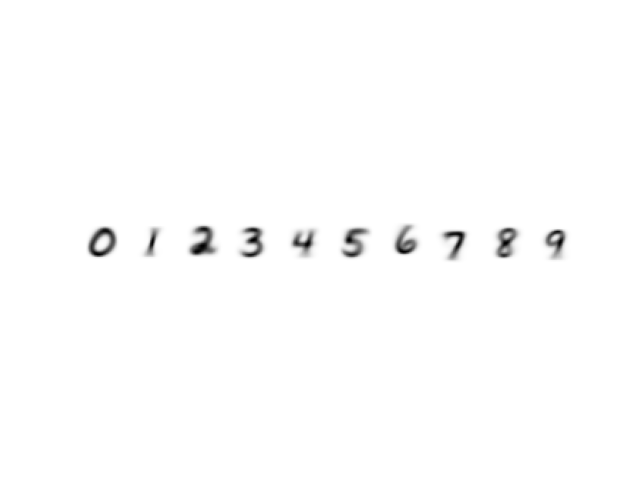
\includegraphics[width=\columnwidth]{images/classMeans.png}
    \caption{Each digit in the dataset drawn with the mean values for each pixel across the training data. %
      \label{fig:classMeans}}
\end{figure}



\section{Solution}
\subsection{model}
The solution for the optical character recognition problem in this project is to use Linear Determinant Analysis (LDA). The features used for the model are the values of the pixels, meaning that the dataset starts with 784 features (because of the 784 pixels per image). The LDA performs a dimensionality reduction, and then uses a linear discrminant to determine the likelihood for each class. The class with the greatest likelihood is predicted to be the class of the datapoint. 

This solution can lower the dimensionality of the data to any amount, and the accuracy (tested against the test data) is shown in fig ~\ref{fig:DimensionBars}


\begin{figure*}
    \centering
    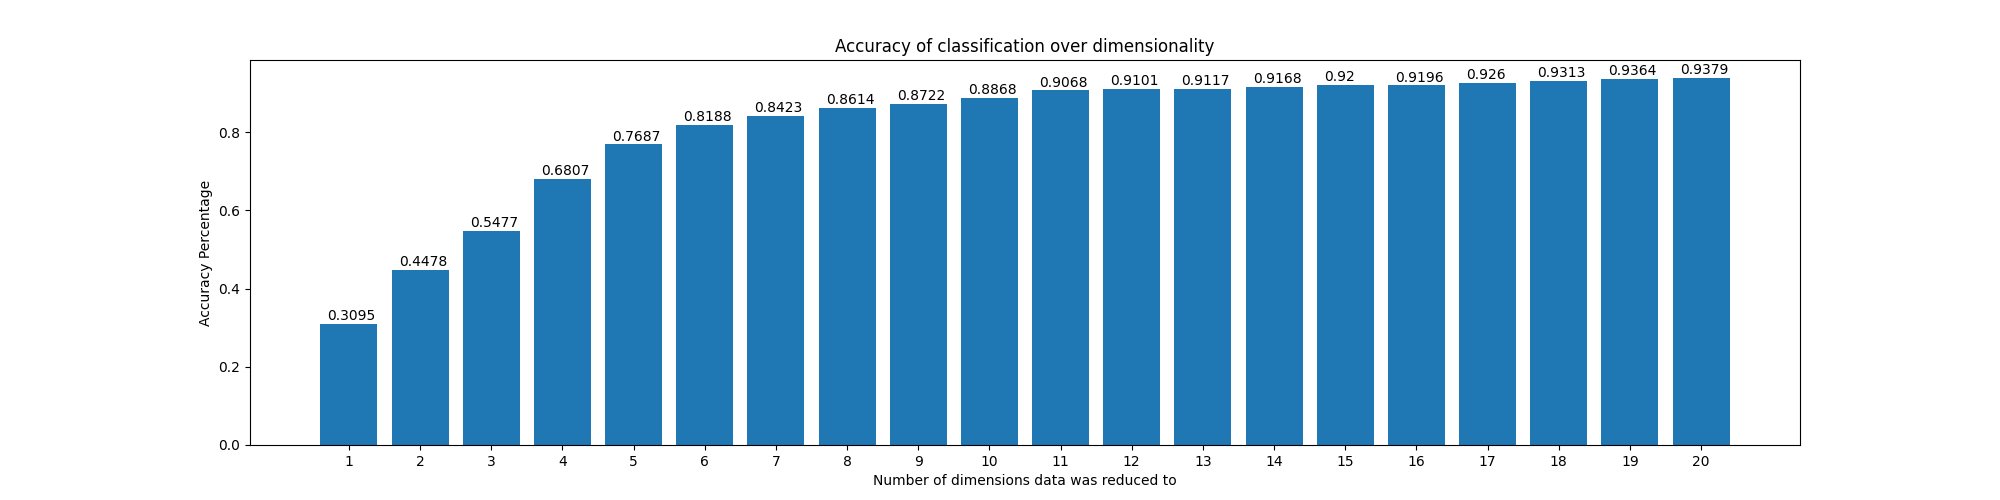
\includegraphics[width=\textwidth]{images/CPUBars.png}
    \caption{Comparison of accuracy across dimensionality reduction. %
      \label{fig:DimensionBars}}
\end{figure*}

\subsection{GPU acceleration}
It is very helpful to have machine learning models train quickly and run quickly. To attempt an acceleration of the training of this LDA model, a GPU was used and compared to using CPU code. The CPU code was implemented using the Python numpy library, and the GPU code used the Python cupy library. The cupy library is incredibly easy to use because it was made to mirror the numpy library so that it could be used as a drop-in replacement for numpy. There were very minor code changes needed to get the training code working on the GPU. Averaged over 10 runs, the CPU code took 28.23 seconds to run, and the GPU training took 3.27 seconds to run, resulting in a speed up by a factor of 8.6. The timer was started after the training data had already been copied to the device memory, and was stopped after the data was copied back to host memory. Accelerating the training on the GPU greatly decreased the training time, and could also be applied to the classification of data after training, but the MNIST dataset does not provide a large enough test data set to where GPU acceleration would provide much benefit. 

Since cupy was able to be used a drop-in replacement for numpy, the code was able to be made configurable for running with a GPU or without a GPU. Inside the jupyter notebook with the code, there is a parameter "globalUseGPU" that can be set to True to use the GPU or False to only use the CPU. If configured to only use the CPU, the code will not need any GPU dependencies to run, and can be run on a machine that does not have a GPU.

System tested on has a AMD Ryzen 9 3900X CPU, and NVIDIA Geforce RTX 3080 Ti GPU. 


\section{Assumptions, Constraints and Implications}

\subsection{ Cenetered Characters}
One massive assumption was found which has to do with the dataset. The dataset contains very well formatted samples, with each handwritten character being well centered in the image. Both the training data and the test data are well formatted like this. This does allow for the model to use the value of each pixel as a feature, since all the data has the pixels for the characters line up. However, if the model is applied to real data that is not well formatted, the predictions are not nearly as accurate. To try the model against some real world data, I had written some characters myself, converted them to the 28x28 pixel format, and put them into the model to get a prediction. For these real data tests, a lower dimensionality of 10 was used, which had an accuracy of 88\% on the test data. When used with images I had created myself, the accuracy was approximatly 10\%, and since there are only 10 classes, that is about as good as a random guess. Why was the model testing to such a high accuracy, but the data I created tested so poorly? This is because of how the pixel values are used as features. Since the color value of each pixel is use as a feature, the model is essentially choosing a prediction based on how similarly the pixel are colored in compared to the classes in the training data. Since the training data is so well formed with centered characters, any data to get a prediction from must also be well formed with centered data for the prediction to be accurate.

So here is a significant constraint of this model: Any data to be predicted must be well formed with the character being centered in the image. To see this constraint in action, see fig ~\ref{fig:shiftedComparison} where the prediction is shown for the test image and the test image shifted to the left. So if this model was to be put to use out in the world, the data would first need to be corrected to be well formatted (meaning the character would have to be centered well in the image) before being fed into the model.

\begin{figure}
    \centering
    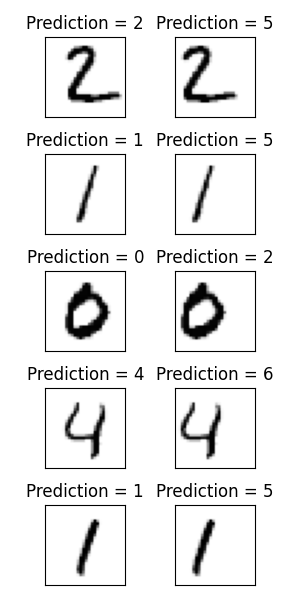
\includegraphics[width=\columnwidth]{images/shiftedComparison.png}
    \caption{A comparison of the predictions made with the origional test image (left) and the same test image shifted to the left by 5 pixels (right). This shows how the model is not robust to images where the character is not centered. Predictions collected with the model having a lower dimensionality of 10.%
      \label{fig:shiftedComparison}}
\end{figure}

\subsection{ Eigenvalues library}
Part of the LDA algorithm is to find the Eigen value and Eigen vectors of a matrix. These values are used to create a map to lower dimensionality. To achieve this, the eig function of the Python numpy linear algebra library (numpy.linalg) was planned to be used. This function will return the eigen values and vectors for a square matrix. However, the cupy Python library was also being used for its ability to run calculation on GPUs. The cupy library has a function that is equivalent to the numpy.linalg.eigh function, but not the numpy.linalg.eig function. The eigh function gets the eigen values and vectors for a complex Hermitian or real symmetric matrix. This function was tested, and the accuracies of the models trained with the eigh function worked just as well or better than the model trained with the eig function. It is not completely known to me what the difference is, but ~\ref{fig:ProjectedTestDataPrediction} and ~\ref{fig:CPUProjectedTestDataPrediction} show the differences of the test data projected to 2 dimensions with the functions.


\begin{figure*}
    \centering
    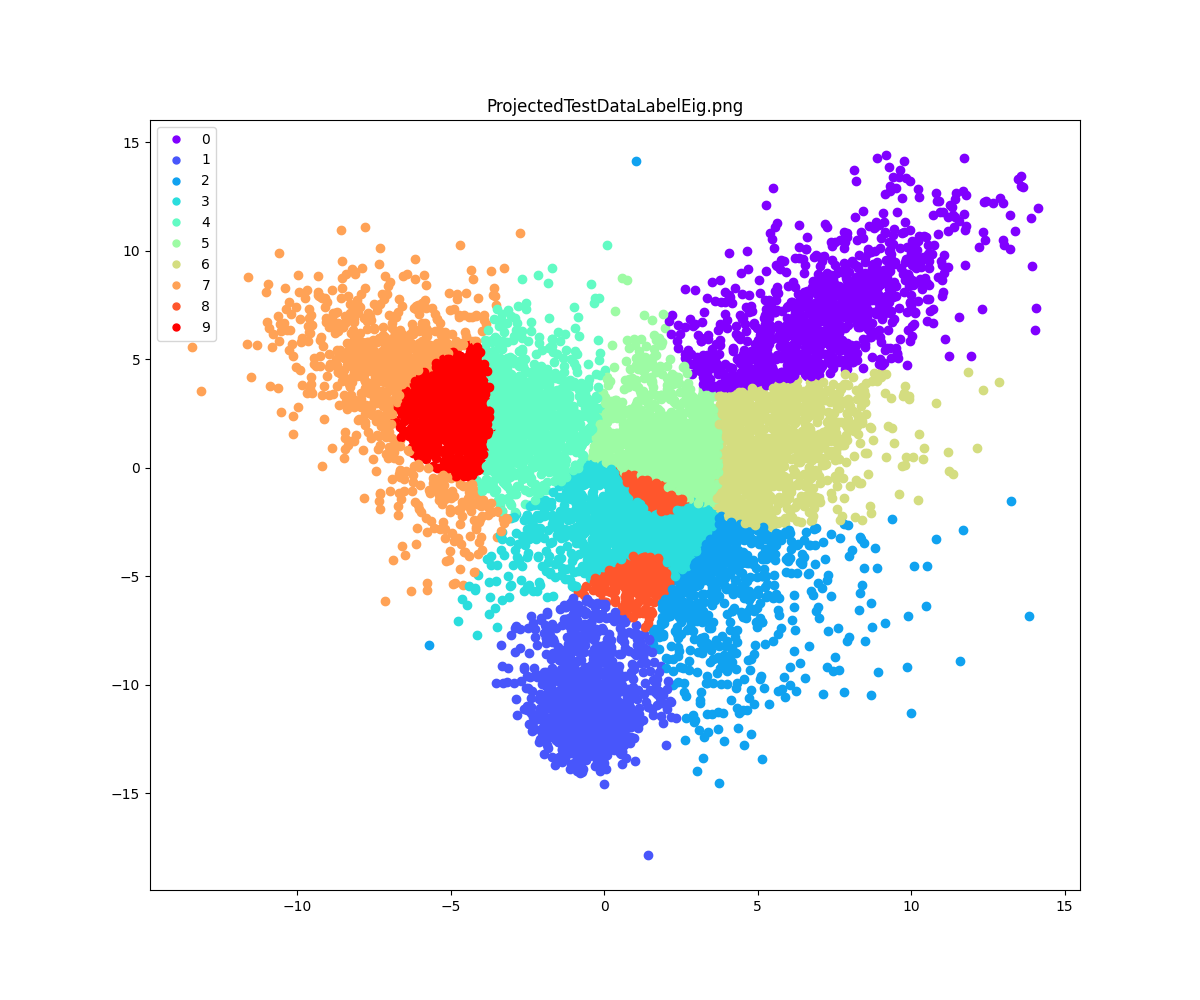
\includegraphics[width=\textwidth]{images/ProjectedTestDataPredictionEig.png}
    \caption{The test data projected to 2 dimensions and colored by the prediction. Generated with the model trained with the numpy.linalg.eig function.%
      \label{fig:ProjectedTestDataPrediction}}
\end{figure*}

\begin{figure*}
    \centering
    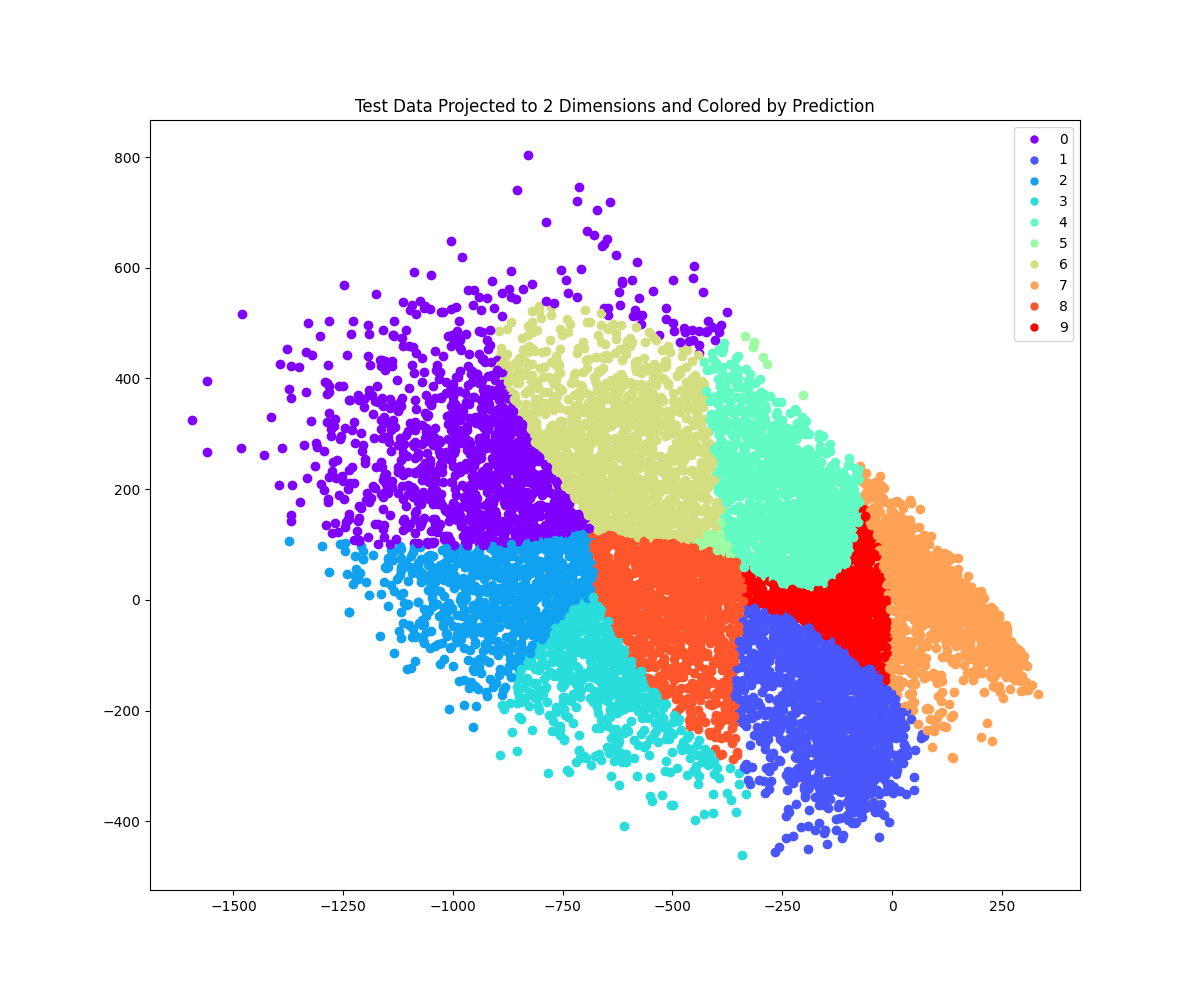
\includegraphics[width=\textwidth]{images/CPUProjectedTestDataPrediction.png}
    \caption{The test data projected to 2 dimensions and colored by the prediction. Generated with the model trained with the (numpy/cupy).linalg.eigh function.%
      \label{fig:CPUProjectedTestDataPrediction}}
\end{figure*}


\subsection{System Setup for GPU}
Setting up the system to run the code with GPU was non-trivial. This was mostly because the system is running windows, and working with CUDA is somewhat challenging on windows. The final configuration of the system was that CUDA and the device driver were installed on windows, and then Windows Subsystem Linux (WSL) was used for the environment to actually run the code. The CUDA toolkit needed to be installed on the WSL, but the device driver only needs to be installed on the host Windows OS. This allowed the CUDA toolkit to be used by the linux environment in WSL and communicated with the device driver on the host Windows OS. Ubuntu was the distro used with WSL.



\section{ Summary}


  \printbibliography
\end{document}